\section{Literature Review}
\label{sec:litreview}

You can mention previous chapters, like Chapter \ref{sec:introduction}, using the label that you have written before.

\subsection{\textbf{Add the title of your subsection here}}
\label{sec:labelname}

\vspace{0.1 in}
\noindent
You can also add labels to a subsection, like in \ref{sec:labelname}




\vspace{0.1 in}
\noindent


Let's add one equation that you can cite in your text \ref{eq:name_of_your_equation}

\vspace{0.1 in}
\noindent

\begin{equation}
\label{eq:name_of_your_equation}
y = mx + n
\end{equation}


\vspace{0.1 in}
\noindent

Let's add a table that you can reference in the text too, Table \ref{table:myparameters}. I prefer to add tables as figures, but they can also be created here in the visual editor very easily or with some latex code.

\begin{table}[H] %  figure placement: here, top, bottom, or page
    \centering
    \caption{Parameters that I use in my experiments}
    \label{table:myparameters}    
    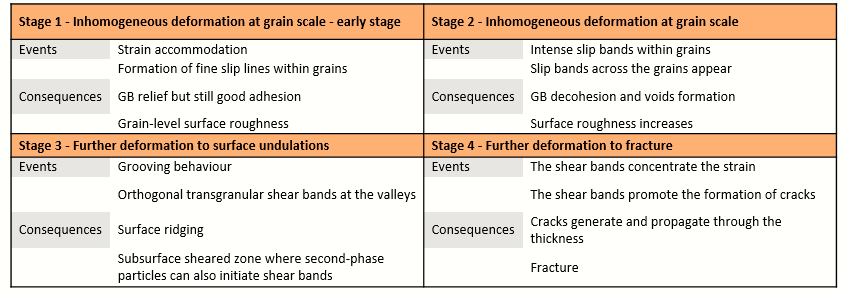
\includegraphics[width=6in]{Figures/LitRev/Stages_table_title.png}
\end{table}

\vspace{0.1 in}
\noindent
You can add Figures too, like in Figure \ref{fig:stages}, with papers cited in the caption.

\begin{figure}[H] %  figure placement: here, top, bottom, or page
    \centering
    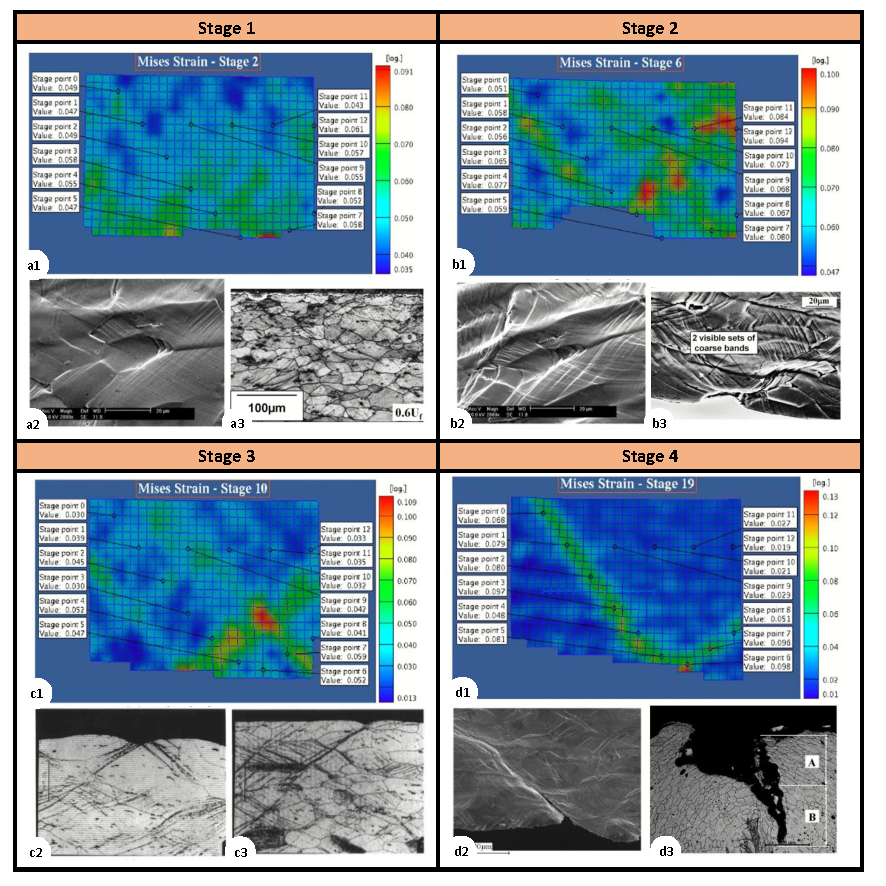
\includegraphics[width=5.5in]{Figures/LitRev/microstructural-features.pdf}
    \caption{Microstructural features at different bending stages from low (a) to high (d) degree of deformation. a1, b1, c1 and d1 are strain maps at the outer sample surface \cite{DAVIDKOV2012} (the outer surface is at the bottom of the maps). a2 \cite{DAVIDKOV2011} and a3 \cite{MATTEI2013}: thin slip lines within the grains. b2 \cite{DAVIDKOV2011} and b3 \cite{MATTEI2013}: wider slip lines and transgranular shear bands. c2 and c3: surface ridging and the subsurface sheared zone \cite{dao2001}. d2 \cite{DAVIDKOV2012} and d3 \cite{DAVIDKOV2011}: cracks that appear and propagate at the outer surface of the sample.}
    \label{fig:stages}
\end{figure}
